Open source repositories are software projects made available through the Internet.\cite{ossWiki}
GitHub is one of the most widely and largely used code host services, with more than ten million repositories.\cite{gitHubWiki}\cite{kalliamvakoupromises} It allows viewing the activity within projects, such as issues, commits and documentation. In recent years, the web site has present an effective way of sharing scientific researches and contributing to them. The great number of public data and the API of GitHub, has made easy for scientists to analyze project data. There are, also, different tools and data domains that support the researchers' tasks.\cite{gandrud2013github}

The \textit{IPython Observatory} project has chosen GitHub as a source of information that will be investigated for the idea of how IPython is used in science. One of the most crucial features of Git that makes it effective to science is the recorded history of changes into a repositories and that they are available to view from everyone\cite{ram2013git}. Furthermore, GItHub presents an option for developers to show their works to colleagues, peers and potential recruiters. A lot of researchers are analysing the usage of programming tools on GitHub and what effect does the version control hosting site has on the improvement of software systems. The Kalliamvakou's paper \cite{kalliamvakoupromises} is investigating possible threats to the validity of researches involving software projects hosted on GitHub. They can be viewed as fundamental steps for analysing all of the repositories connected with IPython notebooks. Figure \ref{fig:perils} is showing the results of the paper. 

\begin{figure*}
\centering
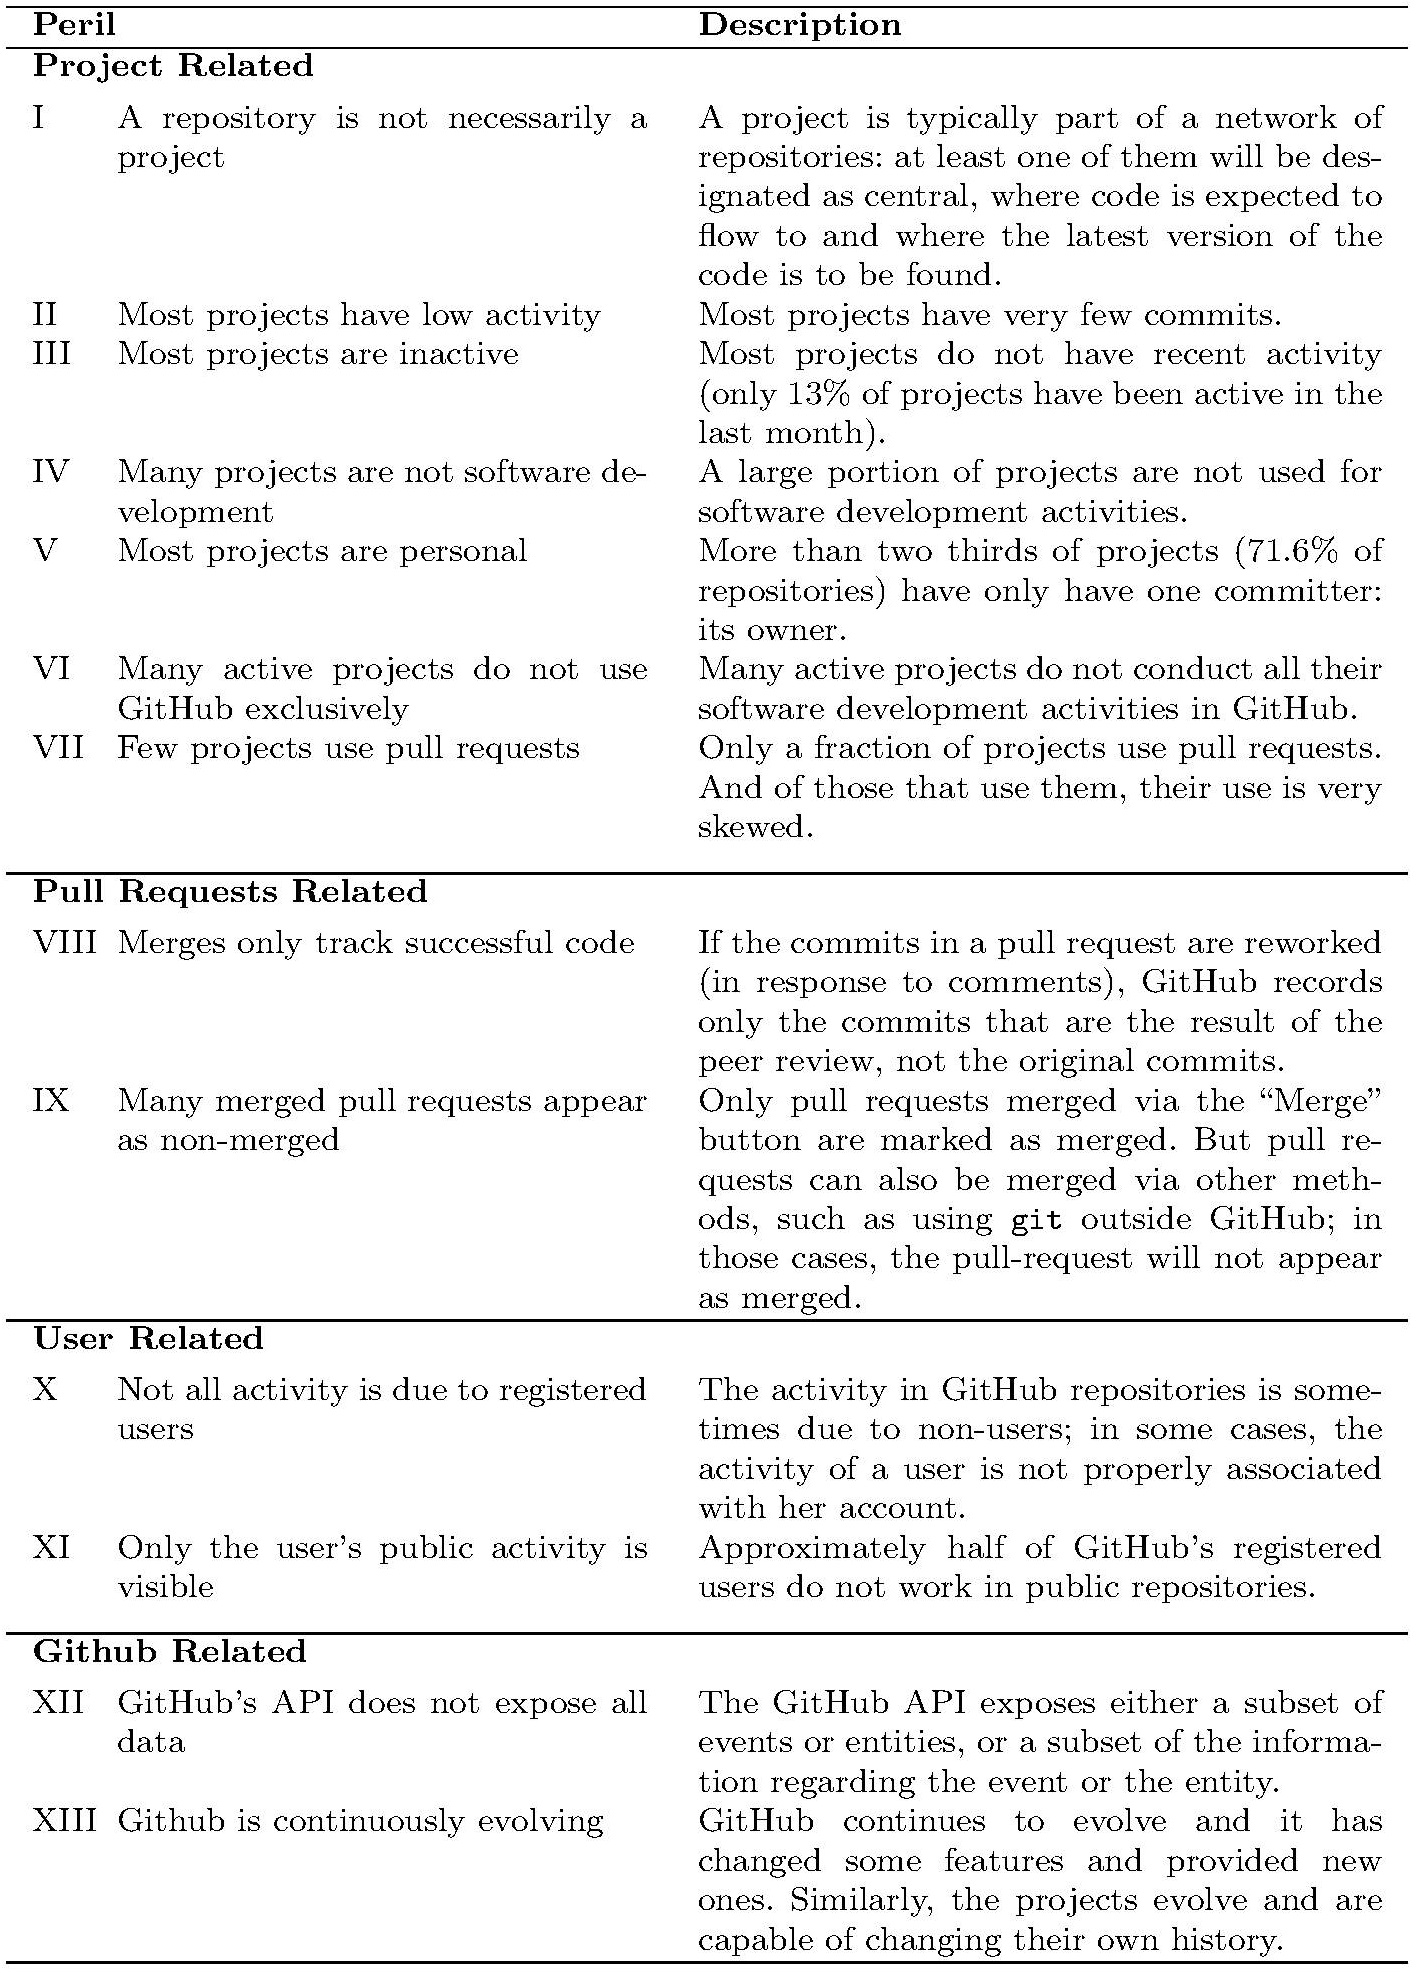
\includegraphics[width=0.7\textwidth]{images/file-page1}
\caption{The Promises and Perils of Mining GitHub Results}
\label{fig:perils}
\end{figure*}